\chapter{Planificación temporal}
\label{chap:planificacion}

La planificación general del proyecto siguiendo un modelo SCRUM, para su aprendizaje, \\ se encuentra en un panel de tareas en Taiga \\ \url{https://tree.taiga.io/project/mgautier-proyecto-fin-de-carrera/backlog}.

Taiga [\ref{subsec:taiga}], es un gestor de proyectos que permite aplicar una metodología de desarrollo ágil SCRUM o Kanban para la realización del mismo.

\begin{figure}[H]
\hspace*{-.2in}{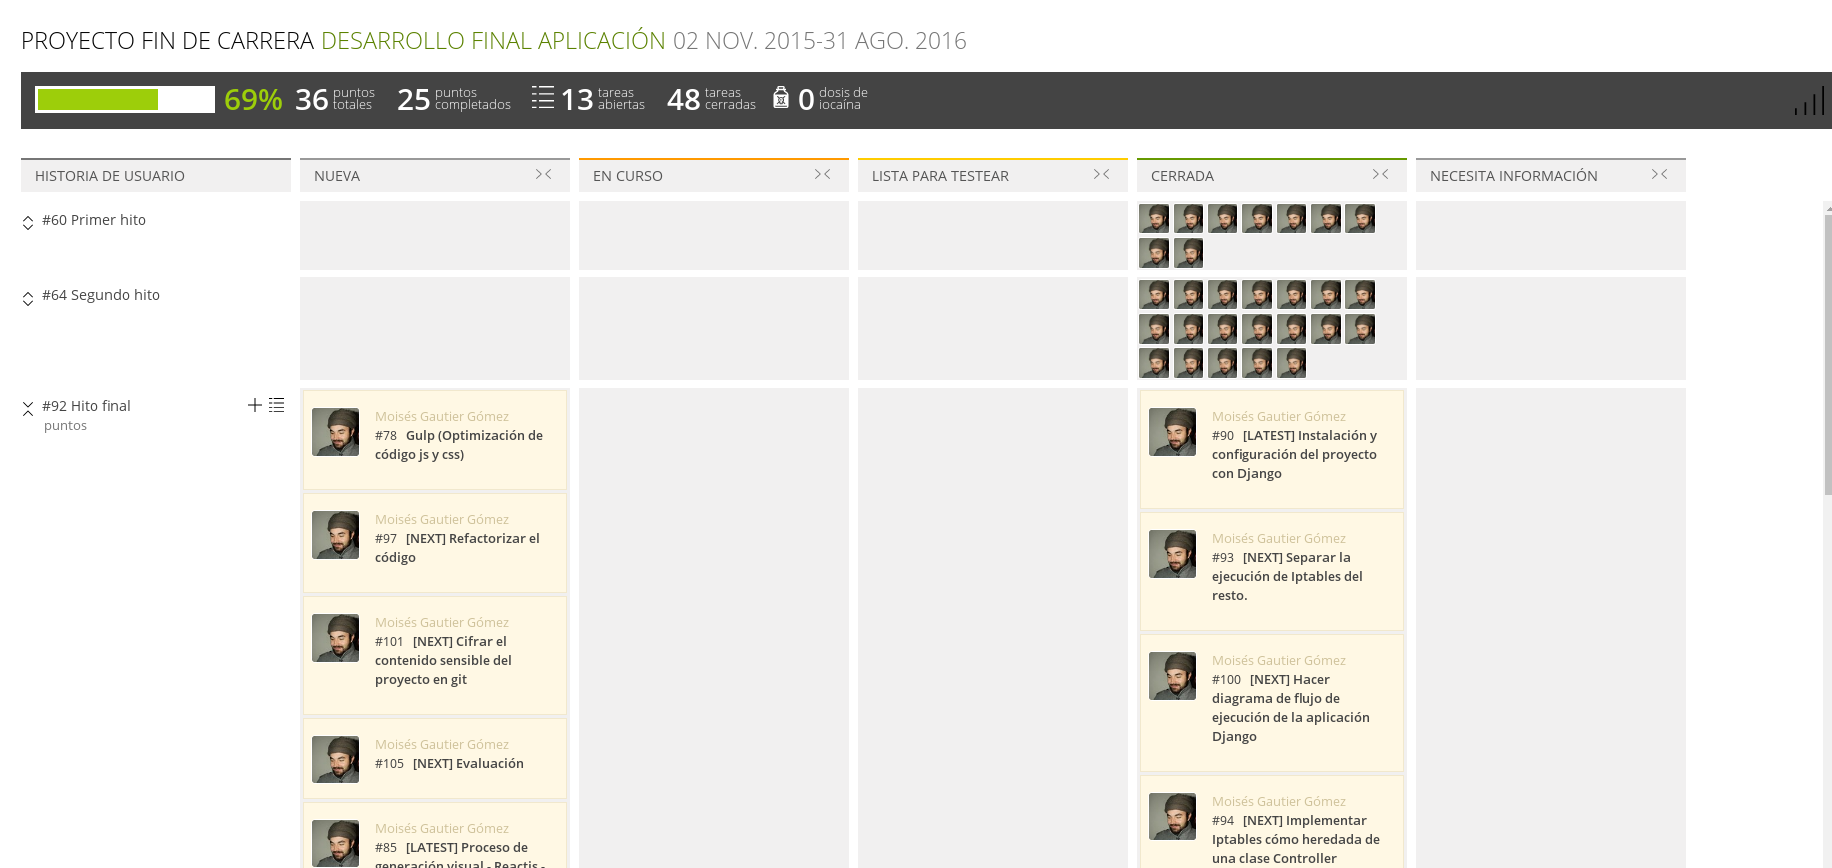
\includegraphics[scale=0.25]{diagramas/hito-taiga.png}}
\caption{Panel de actividades - Taiga}
\end{figure}

Los puntos más importantes del proyecto se han dividido en hitos, así como entregas que se definieron en cada reunión que se realizaba con el director del proyecto. También se ha definido una planificación temporal del desarrollo del proyecto mediante un diagrama de gantt con la duración de las tareas definidas en el panel de actividades de Taiga.\\
\newpage
\sectionmark{Tareas}
\section[Tareas]{Planificación temporal de tareas}
\sectionmark{Tareas}

A continuación se definirán los diferentes hitos que componen el diagrama de Gantt así como las fechas estimadas para los cuales se realizaron los hitos:
\subsection{Hito 1: 1 Mayo a 1 Julio 2015}
\label{subsec:hito1}

En esta primera etapa de desarrollo del proyecto final de carrera, se realizaron los estudios de las tecnologías a implementar, la arquitectura del sistema, las tecnologías de BD, visualización, etc.

\subsection{Hito 2: 1 Julio a 1 Septiembre 2015}
\label{subsec:hito2}

Implementación de los primeros componentes del sistema, como la BD. Definición de las tecnologías finales a implementar después del estudio del estado del arte realizado en el hito anterior. Gestión del código fuente bajo control de versiones Git y estudio de las tecnologías de recogida y correlación de logs con rsyslog. También se diseñan las reglas de filtrado de paquetes para la fuente de seguridad: Iptables.

\subsection{Hito 3: 1 Septiembre a 1 Noviembre 2015}
\label{subsec:hito3}

Se definen las clases del sistema que harán uso de la fuente de seguridad (Iptables, Source, Controller, etc). Se redefine el modelo de la BD.

\subsection{Hito 4: 1 Noviembre 2015 a 1 Enero 2016}
\label{subsec:hito4}

Primera aproximación funcional de la recolección (Pygtail) y correlación de eventos de Iptables en el sistema almacenados en la BD. Una vez la aplicación funciona mediante el uso del terminal se realiza estudio de la mejor forma de adaptar dicha aplicación a formato web con peticiones HTTP para visualizar los eventos generados.

\subsection{Hito 5: 1 Enero a 1 Marzo 2016}
\label{subsec:hito5}

Se decide implementar la solución web con el framework de desarrollo Django para el lenguaje Python. Se realizan los primeros estudios de bibliotecas gráficas que permitan la visualización de eventos en la interfaz web: D3js, C3js, Reactjs, etc.

\subsection{Hito 6: 1 Marzo a 1 Mayo 2016}
\label{subsec:hito6}

Proceso de desarrollo web y generación de visualización de los eventos del sistema en la interfaz web usando la tecnología de C3js y Reactjs. Se comienza a definir la estructura principal de la memoria para disponer de la mayor puntos posibles de cara a una posible defensa en Julio.
\newpage
\begin{minipage}{\linewidth}
  \subsection{Hito 7: 1 Mayo a 1 Julio 2016}
  \label{subsec:hito7}

  Se prosigue con el desarrollo de la memoria y se decide optar por una nueva biblioteca gráfica (Highcharts) para la visualización e interacción de los eventos generados y almacenados en el sistema. Se obtiene una versión definitiva de la aplicación web a falta de la resolución de conflictos en las peticiones ajax de los eventos de la interfaz.

  \subsection{Hito 8: 1 Julio a 19 Septiembre 2016}
  \label{subsec:hito8}

  Refinamiento del modelo de BD para la realización de test de integridad sobre los mismos. Se refactoriza y comenta todos los métodos que tiene la aplicación para facilitar su comprensión al desarrollador futuro. Se finaliza la memoria para la revisión por parte del director del proyecto y su posterior impresión. Se prepara la presentación para la defensa ante tribunal por parte del alumno.
\end{minipage}
\section{Diagrama de Gantt}
\begin{figure}[H]
\hspace*{1.5in}{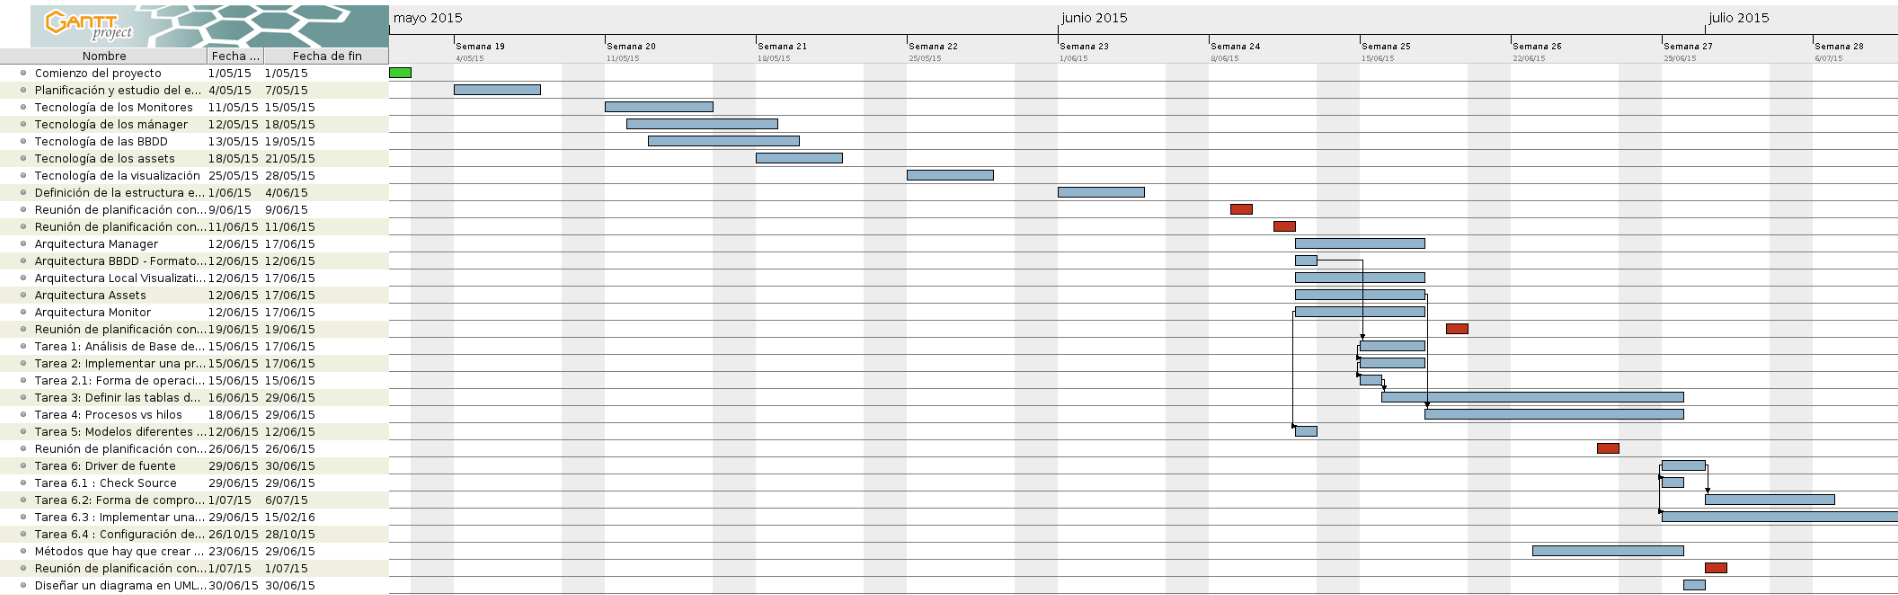
\includegraphics[scale=0.3,angle=270]{diagrama-gantt-hitos/1-mayo-1-julio-2015.png}}
\caption{Hito 1 - \ref{subsec:hito1}}
\end{figure}
\newpage
\begin{figure}[H]
\hspace*{2.75in}{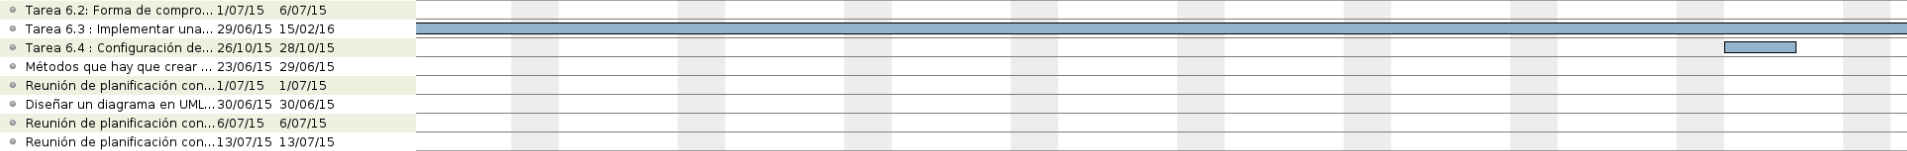
\includegraphics[scale=0.33,angle=270]{diagrama-gantt-hitos/1-julio-1-septiembre-2015.png}}
\caption{Hito 2 - \ref{subsec:hito2}}
\end{figure}
\newpage
\begin{figure}[H]
\hspace*{2.65in}{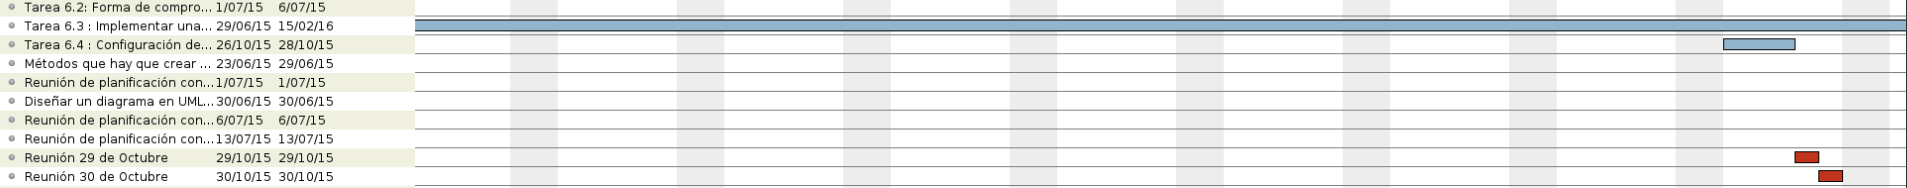
\includegraphics[scale=0.33,angle=270]{diagrama-gantt-hitos/1-septiembre-1-noviembre-2015.png}}
\caption{Hito 3 - \ref{subsec:hito3}}
\end{figure}
\newpage
\begin{figure}[H]
\hspace*{1.5in}{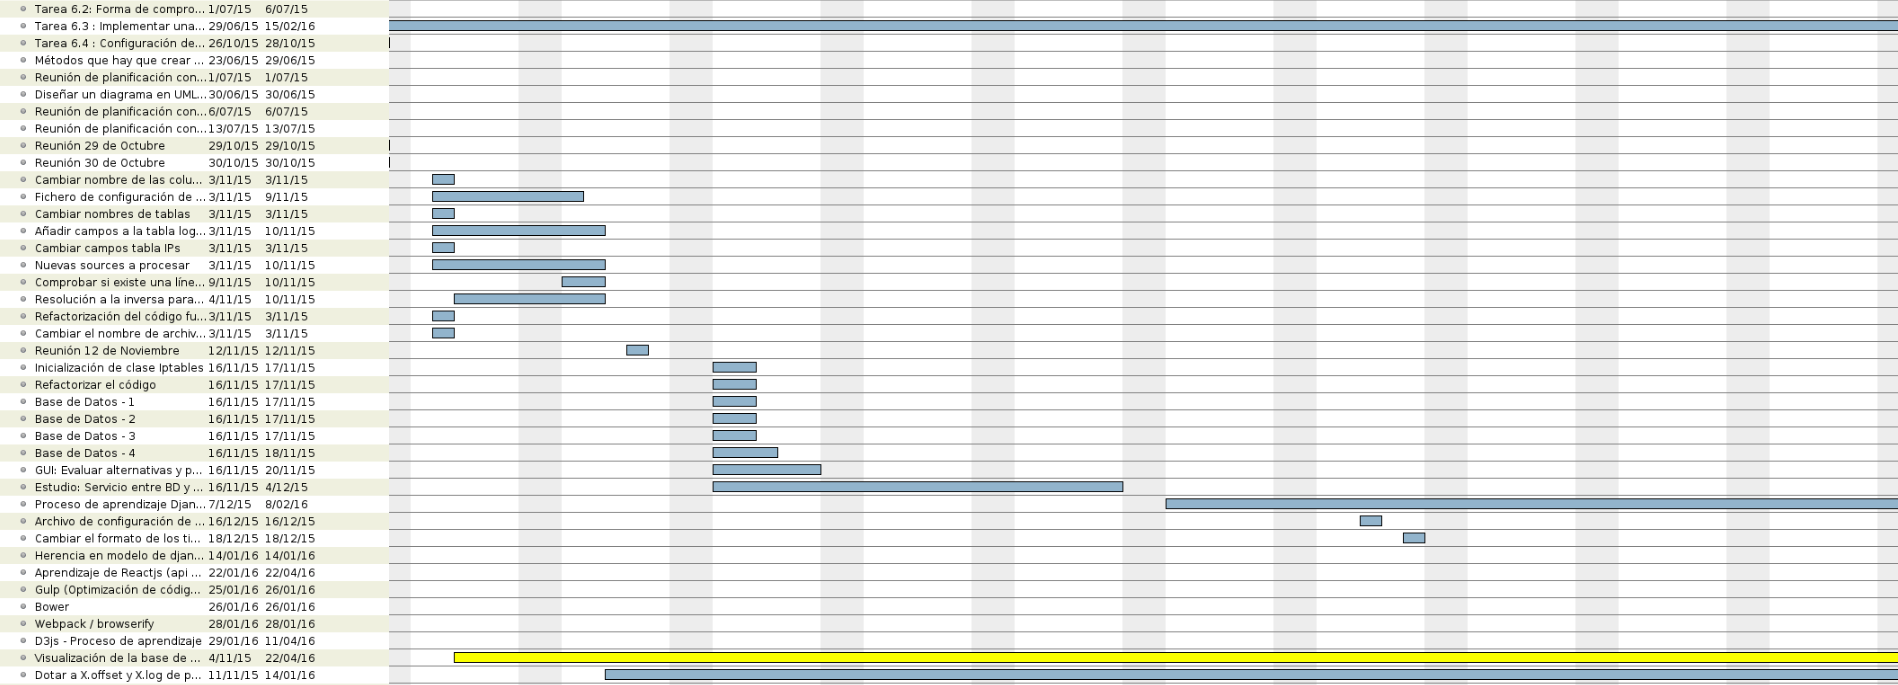
\includegraphics[scale=0.34,angle=270]{diagrama-gantt-hitos/1-noviembre-1-enero-2016.png}}
\caption{Hito 4 - \ref{subsec:hito4}}
\end{figure}
\newpage
\begin{figure}[H]
\hspace*{1.5in}{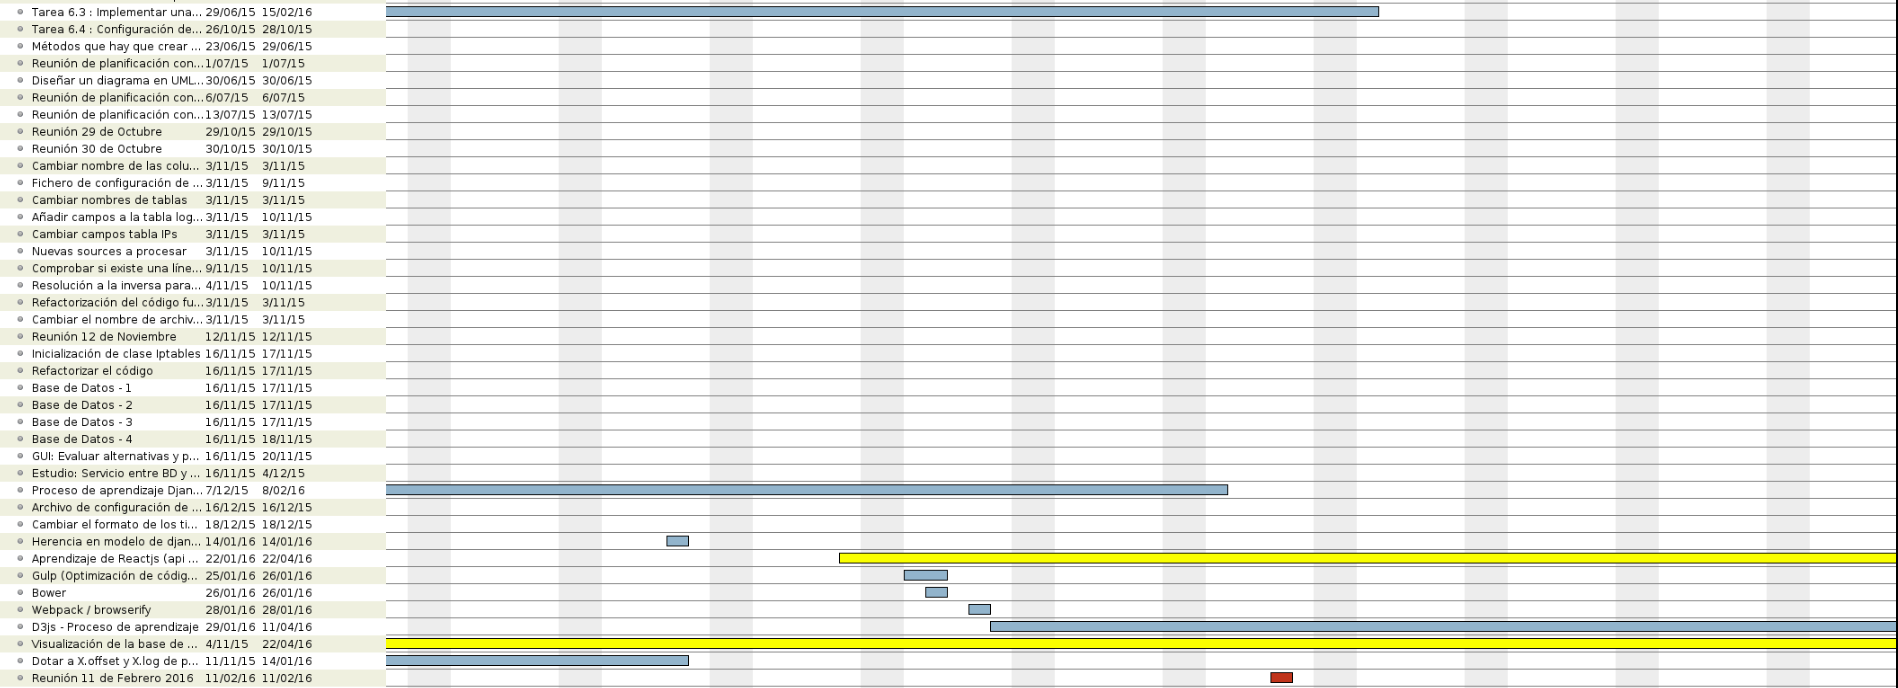
\includegraphics[scale=0.34,angle=270]{diagrama-gantt-hitos/1-enero-1-marzo-2016.png}}
\caption{Hito 5 - \ref{subsec:hito5}}
\end{figure}
\newpage
\begin{figure}[H]
\hspace*{2.5in}{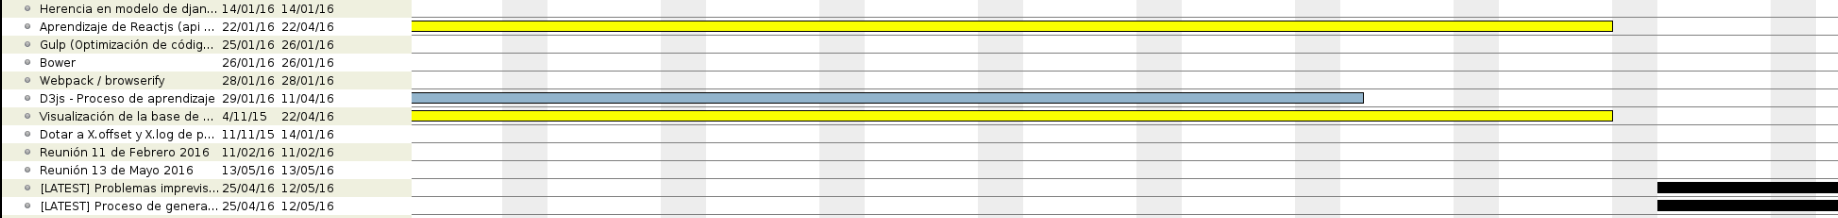
\includegraphics[scale=0.34,angle=270]{diagrama-gantt-hitos/1-marzo-1-mayo-2016.png}}
\caption{Hito 6 - \ref{subsec:hito6}}
\end{figure}
\newpage
\begin{figure}[H]
\hspace*{2.5in}{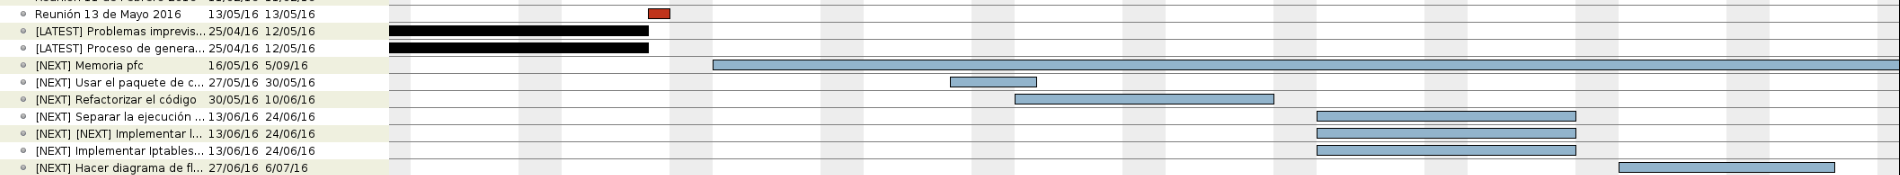
\includegraphics[scale=0.34,angle=270]{diagrama-gantt-hitos/1-mayo-1-julio-2016.png}}
\caption{Hito 7 - \ref{subsec:hito7}}
\end{figure}
\newpage
\begin{figure}[H]
\hspace*{2.5in}{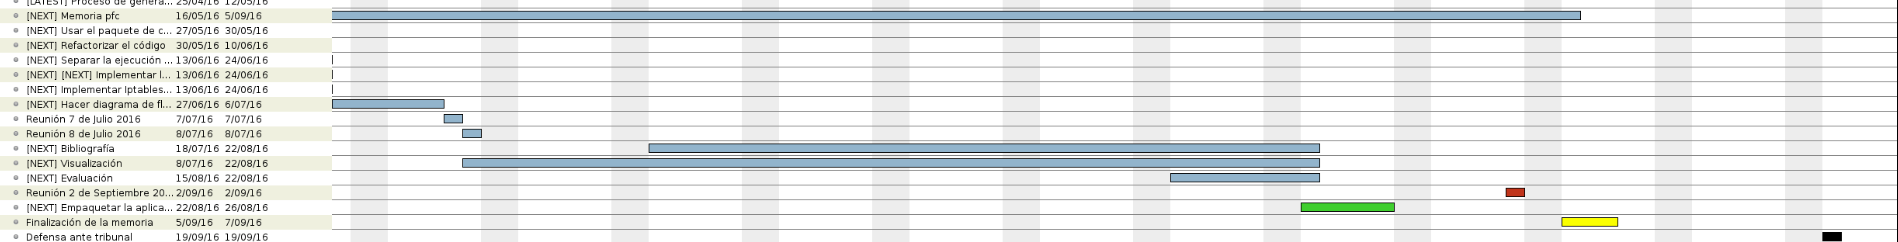
\includegraphics[scale=0.34,angle=270]{diagrama-gantt-hitos/1-julio-19-septiembre-2016.png}}
\caption{Hito 8 - \ref{subsec:hito8}}
\end{figure}
